\documentclass[12pt]{article}
\usepackage[T1]{fontenc}
\usepackage{lmodern}
\usepackage[margin=1in]{geometry}
\usepackage{setspace,amsmath,amssymb,graphicx,booktabs,array,natbib,microtype}
\usepackage[font=small,labelfont=bf]{caption}
\usepackage[hidelinks,breaklinks]{hyperref}
\bibliographystyle{plainnat}
\setcitestyle{authoryear,round,aysep={}}
\onehalfspacing
\emergencystretch=3em
\setlength{\tabcolsep}{4pt}
\renewcommand{\arraystretch}{1.12}
\newcommand{\notes}[1]{\par\vspace{5pt}\begin{minipage}{.98\textwidth}\footnotesize\singlespacing #1\end{minipage}}
\newcommand{\HouseGap}{9.25}
\newcommand{\HouseCI}{[7.17, 11.35]}
\newcommand{\GeoChange}{0.39}
\newcommand{\GeoCI}{[-1.02, 1.60]}
\newcommand{\CondoGap}{0.77}
\newcommand{\CondoCI}{[-0.01, 1.56]}
\newcommand{\InitialGap}{11.42}
\newcommand{\PartyChange}{-2.32}

\newcommand{\FocusedJoint}{9.02}
\newcommand{\FocusedTopSixty}{8.51}
\newcommand{\FocusedPositive}{4.68}

\newcommand{\RobustHuber}{6.73}
\newcommand{\RobustTrimOne}{7.66}
\newcommand{\RobustTrimTwo}{5.15}
\newcommand{\RobustHouseBQHuber}{8.83}
\newcommand{\RobustCondoBQHuber}{-0.49}
\newcommand{\RobustHuberCI}{[5.32, 8.76]}
\newcommand{\RobustCondoBQHuberCI}{[-1.00, -0.03]}
\newcommand{\RobustHouseBQHuberCI}{[7.39, 10.28]}
\newcommand{\RobustHuberDown}{34}
\newcommand{\TailCF}{15}
\newcommand{\TailFF}{4}
\newcommand{\RobustHouseInvQTen}{63}
\newcommand{\RobustMin}{5.15}
\newcommand{\RobustMax}{7.66}

\newcommand{\RelPairs}{358}
\newcommand{\RelPairsStrict}{238}
\newcommand{\RelShareCash}{5.7}
\newcommand{\RelShareFin}{2.3}
\newcommand{\NoRelOLS}{4.87}
\newcommand{\NoRelOLSCI}{[2.69, 6.76]}
\newcommand{\NoRelHuber}{4.02}
\newcommand{\NoRelHuberCI}{[2.28, 5.73]}
\newcommand{\NoRelStrictOLS}{6.71}
\newcommand{\NoRelStrictOLSCI}{[4.69, 8.72]}
\newcommand{\NoRelMin}{2.83}
\newcommand{\NoRelMax}{4.87}
\newcommand{\NoRelChange}{-4.38}
\newcommand{\NoRelChangeCI}{[-5.63, -3.18]}
\newcommand{\CompanyCash}{1.53}
\newcommand{\CompanyCashCI}{[-1.79, 5.44]}
\newcommand{\OtherCash}{13.77}
\newcommand{\OtherCashCI}{[10.96, 15.98]}
\newcommand{\CompanyCashNoRel}{1.55}
\newcommand{\CompanyCashNoRelCI}{[-1.75, 5.49]}
\newcommand{\OtherCashNoRel}{7.11}
\newcommand{\OtherCashNoRelCI}{[4.48, 9.12]}
\newcommand{\NoRelInvQTen}{45}
\newcommand{\NoRelHuberInvQTen}{37}
\newcommand{\RelRatio}{2.5}
\newcommand{\RelShareOfGap}{47}
\newcommand{\OtherMinusCompanyNoRel}{5.56}
\newcommand{\OtherMinusCompanyNoRelCI}{[0.97, 9.07]}
\newcommand{\RelGrowthCFRel}{0.65}
\newcommand{\RelGrowthCFUnrel}{0.34}
\newcommand{\RelGrowthFCRel}{0.27}
\newcommand{\RelGrowthFCUnrel}{0.20}
\newcommand{\PartyShareA}{98}
\newcommand{\PartyShareZ}{99}
\newcommand{\CashCompanyPairs}{794}
\newcommand{\SwitchPairs}{1,781}

\newcommand{\CondoFlagged}{189}
\newcommand{\CondoFlaggedStrict}{137}
\newcommand{\CondoNoRel}{-0.46}
\newcommand{\CondoNoRelCI}{[-1.16, 0.14]}
\newcommand{\CondoNoRelStrict}{-0.26}
\newcommand{\CondoNoRelStrictCI}{[-0.97, 0.34]}
\newcommand{\CondoRelChange}{-1.23}
\newcommand{\CondoRelChangeCI}{[-1.71, -0.82]}
\newcommand{\CondoBootCI}{[-0.02, 1.55]}
\newcommand{\CondoDeedEnds}{13,092}
\newcommand{\CondoEnds}{13,168}
\newcommand{\CondoAmbiguous}{31}
\newcommand{\HouseBQFlagged}{449}
\newcommand{\HouseBQNoRel}{7.50}
\newcommand{\HouseBQNoRelCI}{[6.00, 9.19]}
\newcommand{\AddrPairs}{1,595}
\newcommand{\AddrRemaining}{4,053}
\newcommand{\AddrOLS}{3.76}
\newcommand{\AddrOLSCI}{[1.16, 6.05]}
\newcommand{\AddrChange}{-1.11}
\newcommand{\AddrChangeCI}{[-2.76, 0.29]}
\newcommand{\AddrPersonOLS}{4.41}
\newcommand{\AddrPersonOLSCI}{[2.14, 6.75]}
\newcommand{\AddrShareCash}{16.7}
\newcommand{\AddrShareFin}{17.2}

\newcommand{\DeedN}{40}
\newcommand{\DeedYes}{16}
\newcommand{\DeedShare}{40}
\newcommand{\DeedCI}{[26, 55]}
\newcommand{\DeedPossible}{9}
\newcommand{\DeedShareWithPossible}{62}
\newcommand{\DeedBoxA}{13}
\newcommand{\DeedUN}{20}
\newcommand{\DeedUYes}{2}
\newcommand{\DeedUShare}{10}
\newcommand{\DeedUCI}{[3, 30]}
\newcommand{\DeedUBoxA}{1}

\title{\bfseries Who Gets the House?\\[2mm]\large Related-Party Transfers and the Cash--Mortgage Price Gap in New York City}
\author{Pablo Loschi\thanks{Independent researcher, Berlin, Germany. Correspondence: \texttt{loschi.pablo@gmail.com}. ORCID: \href{https://orcid.org/0009-0004-9455-4713}{0009-0004-9455-4713}. This research received no external funding. The author reports no relevant financial interests or positions and no outside rights to review the research before dissemination.}}
\date{24 September 2026\\\small Working paper, version 3.1}
\begin{document}
\maketitle
\begin{abstract}\singlespacing\noindent
Cash buyers are widely believed to pay less because their offers are certain to close. I examine that reading with repeat sales of New York City houses and condominiums sold in 2016--2025 and linked to deed and mortgage records. Financed purchases of houses are associated with prices \HouseGap{} log points above cash purchases of the same house, after permit, institutional-seller, party-type and ZIP-year controls. The gap depends on who pays cash. When the cash buyer is a company, it is \CompanyCash{} log points, with an interval that includes zero. Deeds on which the seller and buyer share a surname, a marker of possible transfers between relatives, are \RelShareCash{} percent of unfinanced and \RelShareFin{} percent of financed sales, and in a random sample \DeedShare{} percent of their transfer reports show a non-market sale, against \DeedUShare{} percent for other cash deeds. Excluding the \RelPairs{} pairs that contain one reduces the house gap to \NoRelOLS{} log points \NoRelOLSCI{}. With the same screen applied to both property types under a common design, the house contrast is \HouseBQNoRel{} log points and the condominium contrast \CondoNoRel{}. At an assumed 10 percent failure rate, even the reduced house gap would require a loss of \NoRelInvQTen{} percent of the price on a failed sale to be a pure premium for execution certainty. Much of the measured cash discount reflects who buys with cash rather than what closing certainty is worth, which cautions against using it to calibrate taxes or subsidies on the payment method.
\end{abstract}
\noindent\textit{JEL:} G21, G51, R21, R31.\quad\textit{Keywords:} cash purchases; mortgage finance; related-party transfers; execution risk; repeat sales; New York City.
\newpage

\section{Introduction}
Buyers who pay cash often pay less. Across United States markets the mortgage--cash price difference is on the order of ten percent \citep{reher2024}, and \citet{hanhong2024} link a smaller Los Angeles cash discount to the risk that a financed closing fails. The usual reading is that sellers accept less in exchange for certainty. The alternative is composition: cash purchases may differ in the properties, circumstances and parties involved, so that the average gap says more about who pays cash than about what certainty is worth. The distinction matters for policy. Proposals to tax cash purchases, or to offset the cash buyer's advantage, take the gap as a measure of that advantage.

This paper measures the gap in New York City, where public deed and mortgage records can be linked to repeat sales and where financed buyers also bear a statutory mortgage recording tax of 1.80 to 1.925 percent of loan principal. An archived panel covers house and condominium sales in Manhattan, the Bronx, Brooklyn and Queens between 2016 and 2025. The financing contrast compares the appreciation of properties that switch from a cash to a financed purchase with those that switch the other way. It is estimated jointly with permit restrictions, institutional-seller exclusions, buyer and seller type controls and ZIP-year effects, and every change in specification is evaluated with a common parcel bootstrap.

For houses the contrast is \HouseGap{} log points, with bootstrap interval \HouseCI{}, and between \RobustMin{} and \RobustMax{} log points under estimators that limit the weight of extreme appreciation. Record-consistency restrictions, borough omissions and alternative financing windows leave it positive throughout. Condominiums behave differently: under a common borough-quarter design their contrast is \CondoGap{} log points \CondoCI{}, and slightly negative under robust estimators.

The main new result is that the house gap belongs to particular cash buyers rather than to cash. When the buyer at the unfinanced sale is a company, the contrast is \CompanyCash{} log points \CompanyCashCI{}. When it is an individual or another party, it is \OtherCash{} \OtherCashCI{}. Deed party names identify one reason. Sales on which the grantor and grantee share a surname, a marker of possible transfers between relatives, which need not be priced at arm's length, make up \RelShareCash{} percent of unfinanced sale endpoints and \RelShareFin{} percent of financed ones. Because such transfers sit on the cash side of both switching arms, they raise measured appreciation in cash-to-financed pairs and lower it in financed-to-cash pairs. That inflates the contrast while leaving the symmetry diagnostic of Section~\ref{sec:sym} unchanged. Excluding the \RelPairs{} pairs with a same-surname deed changes the house contrast by \NoRelChange{} log points \NoRelChangeCI{}, to \NoRelOLS{} \NoRelOLSCI{}. Ignoring the 40 most common surnames to limit coincidental matches gives \NoRelStrictOLS{} \NoRelStrictOLSCI{}. The flag is a proxy: it misses relatives with different surnames and can match unrelated people, and the change it produces is not an estimate of the share of the gap caused by family transfers. A reading of the state transfer reports filed with a random sample of deeds supports it: \DeedShare{} percent of flagged deeds \DeedCI{} declare a sale between relatives, a buyer who is also a seller or a non-standard deed, or report a zero price with no transfer tax, against \DeedUShare{} percent \DeedUCI{} of other cash deeds. Applied to both property types under a common design, the screen moves the house contrast from \InitialGap{} to \HouseBQNoRel{} log points and the condominium contrast from \CondoGap{} to \CondoNoRel{} \CondoNoRelCI{}, so the divergence between property types survives. Also excluding deeds on which the grantor and grantee share a mailing address lowers the house contrast further to \AddrOLS{}, but that additional change, \AddrChange{} \AddrChangeCI{}, is not distinguishable from zero.

The divergence between property types and between cash buyers bears on the execution-risk reading. A seller indifference condition converts a contrast into the loss a seller would have to expect on a failed financed sale if the entire contrast were a premium for execution certainty. At an assumed 10 percent failure probability, the headline house contrast implies a loss of 87 percent of the price, and the contrast without same-surname transfers \NoRelInvQTen{} percent, compared with about 7 percent for condominiums. These figures describe what execution risk would have to explain, not its share, because failure probabilities and continuation values are unobserved. Financing-specific associations with mortgage rates and inventory, which an execution-risk mechanism would predict, do not survive financing-specific time trends.

The paper makes three contributions. It applies one repeat-sales design to houses and condominiums in the same city and finds the contrast concentrated in houses. It shows that the house contrast depends on the identity of the cash buyer, and that excluding same-surname deeds, which administrative financing labels inherit from the deed record, reduces the measured contrast by almost half. And it evaluates each threat (renovation, distress, party composition, local appreciation, record errors and extreme growth) by refitting the joint model with paired uncertainty. \citet{hanhong2024} observe listings, agreement dates and relisting, which this paper cannot. \citet{reher2024} attribute much of the national mortgage--cash premium to heterogeneity in sellers' circumstances and beliefs; the buyer-identity results here point to the same kind of heterogeneity from the buyer side. Repeat sales remove fixed property attributes \citep{bailey1963} but not changes in condition or transaction circumstances, and distressed sales, which trade at substantial discounts \citep{campbell2011}, are addressed through institutional-name exclusions and a document-level pilot.

The paper does not observe contracts, contingencies or failed closings. Its financing labels come from record linkage rather than verified loan purpose, and its surname flag is a proxy for a relationship, not a legal finding; Section~\ref{sec:conclusion} collects these limits. It does not estimate the incidence of the mortgage recording tax or responses to New York's 2019 transfer-tax thresholds. Those statutory questions are analysed in a companion paper \citep{loschi2026shape}, which reports no repeat-sales estimates.

\section{Financing institutions in New York City}
\subsection{The recording tax and ownership form}
New York Tax Law Article 11 taxes mortgages of real property (\citealp{nytaxlaw,nycmrt2026}). Sections 253 and 253-a, together with the city schedule, produce standard borrower rates of 1.80 percent below \$500,000 of mortgage principal and 1.925 percent at or above that amount for the covered residential categories. A qualifying lender generally pays the separate 0.25 percent special additional tax; exemptions and instrument-specific credits can change the amount due. Section 253(2) excludes the first \$10,000 of principal for qualifying one- and two-family residences, reducing that component by \$30. These rules are distinct from transfer taxes on the sale price.\footnote{Primary sources: New York Tax Law \S\S253, 253-a, and the NYC Department of Finance mortgage recording tax schedule. The analysis does not reconstruct individual mortgage tax returns.}

For illustration, a standard \$720,000 mortgage used to buy a \$900,000 condominium implies a borrower recording charge of \$13,860 before any applicable instrument-specific credits. A cash purchase records no purchase mortgage. A co-operative share loan is secured by personal property rather than a mortgage on an individually owned real-property unit, so it does not attract the same tax. This does not make a co-operative purchase exempt from all transfer taxes or other closing charges.

The distinction is statutory. Sellers' prices, financing terms and ownership choices can respond, so statutory borrower liability is not an estimate of the ultimate economic burden. The same boundary creates a measurement problem: searching real-property mortgages alone cannot identify co-operative share financing. ACRIS personal-property filings must be investigated separately.

\section{Data and record linkage}
\subsection{Samples and the boundary of replication}
The repeat-sales input contains 290,840 archived observations across five boroughs. Excluding Staten Island leaves 166,907 house and 82,488 condominium sales. The exclusion reflects the coverage of the ACRIS linkage used here; it is not a claim that Staten Island has the same financing measurement.

The panel-construction code combines NYC Department of Finance annualized sales with ACRIS real-property master and legal records. Condominium billing lots can differ from the unit lots on which deeds and mortgages are recorded. The archived code recovers a unique deed through borough, block, consideration and date before assigning the unit parcel. The four archived input files are byte-identical to repository commit \texttt{f404e48320a81e3bfe20127af2ed7c2d9fb5268e} (\citealp{loschicode2026}). All estimates are recomputed from that archived panel; its record matches are documented but not independently re-verified.

New public extracts add DOB permit dates, PLUTO geography, ACRIS deed parties and consideration, co-operative transactions and personal-property filings. The source agencies are cited explicitly (\citealp{nycsales2026,acrisrp2026,acrispp2026,dob2026,pluto2026,pmms2026}). Source identifiers, preserved extracts, software versions and the exact computational boundary are documented in the replication README. The replication run starts from the archived panel and rebuilds every enrichment and analysis from the preserved public extracts; the raw-to-panel linkage is documented but not re-executed.

\subsection{Financing and repeat-sale construction}
For houses and condominiums, financing is the archived indicator of a matched purchase-window mortgage. The strict, base and wide windows are respectively $[-15,+30]$, $[-15,+90]$ and $[-15,+180]$ days around the sale, using document dates with recording-date fallback in the panel-construction code. Narrow, base and wide labels are retained. The absence of a matched mortgage is referred to as cash for brevity, but can include unobserved borrowing, missed linkage or instruments outside the rule. Assignments and satisfactions must not be counted as new purchase mortgages.

Within each eligible house or condominium parcel, sales are sorted by date and adjacent observations at least 1,095 days apart are retained. This yields 8,208 house pairs and 6,584 condominium pairs. All sales fall between 2016 and 2025; in the headline house sample, first sales run from January 2016 to December 2022 and resales from March 2019 to December 2025. Adjacency is established within the archived, already restricted panel; it does not prove that no excluded underlying transfer occurred. Repeated unit sales in co-operatives require an additional unit identifier and follow the broader adjacency audit described below.

The permit restriction removes a house pair if a recorded permit issuance lies between its two sale dates, including endpoints. It leaves 6,316 pairs. Permits measure recorded work, not its cost, completion or quality. Unpermitted work can remain, while some permitted work has little bearing on value. The restriction is consequently a condition sensitivity, not a constant-quality guarantee.

\subsection{Parties, consideration and geography}
Each house endpoint is assigned a deed only when the closest candidate document date within 45 days is unique. Ties remain unresolved. A consideration sensitivity additionally requires a positive deed amount within the greater of one dollar or one percent of the DOF sale price. This checks agreement across records without establishing that consideration equals a negotiated retail value.

Grantor and grantee names supply entity, trust/estate and unknown-party indicators. Explicit company forms take precedence over trust tokens. The narrower institutional rule identifies named financial institutions; a broader alternative also uses generic lending and servicing terms. A pair is excluded when either party is flagged at either date. These rules identify institution-associated transactions, not legally adjudicated foreclosure, deed-in-lieu or REO status. A four-case instrument pilot, reported in Appendix~\ref{sec:pilot}, distinguishes a referee foreclosure transfer from a subsequent lender resale and confirms that ordinary DEED metadata can cover foreclosure instruments. The pilot does not validate the remaining name classifications. Natural-person residual categories likewise do not establish beneficial ownership. The same party records supply the same-surname flag of Section~\ref{sec:who}.

PLUTO version 26v2 supplies a fixed geographic crosswalk for 8,167 house pairs. After the preceding cumulative restrictions, geography reduces the sample from 6,033 to 6,006 pairs. The full specification spans 137 ZIP codes and 52 community districts. Current identifiers provide location controls rather than historical measures of building condition. Of 1,227 ZIP-year endpoint cells, 353 have fewer than five endpoints; fine geographic adjustment comes with limited support in some cells.

\section{Measuring financing-associated price gaps}
\subsection{The joint estimator}
For pair $i$ with sale dates $a$ and $z$, define $y_i=\log P_{iz}-\log P_{ia}$. Let $Q_i$ contain indicators for cash-to-financed ($cf$) and financed-to-cash ($fc$) transitions. The nuisance design $X_i$ contains changes between sale dates in borough-quarter indicators, with optional local-year and party-type terms. The joint regression is
\begin{equation}\label{eq:joint}
y_i=X_i\gamma+Q_i\beta+\varepsilon_i,\qquad
\widehat\pi_J=\tfrac12(\widehat\beta_{cf}-\widehat\beta_{fc}).
\end{equation}
Same-financing pairs help estimate the market controls and provide the switching coefficients' reference. All fixed effects enter in first differences; no interpretation is attached to individual coefficients in a redundant nuisance design. Sparse least squares projects onto that design, with numerical convergence checks.

A simpler statistic residualizes only the outcome and compares switching-group means. With $M_X$ the residual maker and
\begin{equation}
c_i=\tfrac12\left(\frac{1\{cf\}_i}{N_{cf}}-\frac{1\{fc\}_i}{N_{fc}}\right),
\end{equation}
it is $\widehat\pi_R=c'M_Xy$. In contrast, the joint coefficients satisfy $\widehat\beta=(Q'M_XQ)^{-1}Q'M_Xy$. Residualizing $y$ does not also residualize the financing indicators. The two estimands can therefore respond differently when market controls change. Table~\ref{tab:cumulative} reports both, but only equation~\eqref{eq:joint} is the financing coefficient in a jointly controlled regression, and all comparisons use it.

Neither estimator is automatically causal. Within-property differencing removes fixed attributes but leaves time-varying condition, credit access, bargaining circumstances and selection into financing. Permits, recorded party types and local appreciation address observed parts of those differences. They do not make financing exogenous.

\subsection{What symmetry diagnoses}\label{sec:sym}
Suppose the two residual switching means can be written as
\begin{equation}\label{eq:sym}
\mu_{cf}=\pi+u_{cf},\qquad \mu_{fc}=-\pi+u_{fc}.
\end{equation}
Then their half-difference is $\pi+(u_{cf}-u_{fc})/2$, while their sum $A=u_{cf}+u_{fc}$. A small $A$ restricts the sum of the omitted components, not their difference. Opposing condition or composition effects can cancel in $A$ while biasing the half-difference.

This connects the permit and institution analyses. Permits address recorded changes to the property; party records address who transacts and under what observable institutional circumstances. An institution acquiring title without a new mortgage can enter a cash group even when the transfer arises from debt resolution. A small aggregate asymmetry cannot distinguish that composition from renovation. Each restriction must therefore be evaluated through a refitted model and paired uncertainty, rather than treated as validation of the other.

\subsection{Cumulative evidence and neighbourhood appreciation}
Table~\ref{tab:cumulative} gives one specification sequence. The institutional exclusion increases the permit-free gap, whereas buyer and seller type controls reduce it. This difference matters: the name-based exclusion does not explain the positive house contrast, and the party-control change is not a causal decomposition of that contrast.
\begin{table}[htbp]
\centering\small\singlespacing
\caption{Cumulative house robustness}\label{tab:cumulative}
\begin{tabular}{lrrrr}
\toprule
Specification & Pairs & Residual & Joint & Joint 95\% CI \\
\midrule
Original sample & 8,208 & 11.14 & 11.42 & [9.60, 13.19]* \\
Permit-free & 6,316 & 9.34 & 9.63 & [7.80, 11.56]* \\
+ Named institutions excluded & 6,033 & 10.48 & 10.82 & [8.96, 12.67] \\
+ Buyer/seller type controls & 6,033 & 7.23 & 8.50 & [6.58, 10.42] \\
Same geography-linked sample & 6,006 & 7.56 & 8.87 & [6.81, 10.84]* \\
+ Community-district/year & 6,006 & 7.47 & 9.50 & [7.66, 11.33] \\
+ ZIP/year & 6,006 & 6.39 & 9.25 & [7.17, 11.35]* \\
\bottomrule
\end{tabular}
\notes{All estimates and intervals are log points. Every row includes borough-quarter effects. The last two rows are alternative geographic specifications added to the same linked baseline. Institutional exclusions use grantor and grantee name rules at both dates, not verified distress. Stars denote percentile intervals from 999 common parcel-bootstrap refits; other intervals use joint parcel influence functions (CR0). Intervals are pointwise. The residual and joint columns are different estimands.}
\end{table}


The geography-linked baseline holds the sample fixed before adding local-year controls. Community-district-year and ZIP-year effects are alternatives, each supplementing borough-quarter effects. The final joint estimate is \HouseGap{} log points, with bootstrap interval \HouseCI{}. The corresponding residual statistic is smaller, but is not the coefficient of financing in the same jointly controlled regression.

Table~\ref{tab:paired} evaluates changes using their covariance. ZIP-year effects change the joint estimate by \GeoChange{} log points, with interval \GeoCI{}. The data therefore do not establish that local appreciation explains a positive portion of the joint house gap. They also do not rule out every economically meaningful local-composition contribution. Current geography, sparse cells and omitted time-varying characteristics limit that conclusion.
\begin{table}[htbp]
\centering\small\singlespacing
\caption{Paired changes in the joint house contrast}\label{tab:paired}
\begin{tabular}{lrr}
\toprule
Comparison & Change & 95\% CI \\
\midrule
Party controls & -2.32 & [-2.98, -1.65] \\
Community-district/year & 0.63 & [-0.12, 1.38] \\
ZIP/year & 0.39 & [-1.02, 1.60] \\
Original to final & -2.17 & [-4.02, -0.36] \\
\bottomrule
\end{tabular}
\notes{Log points. Differences use cross-specification covariance on original parcel clusters. ZIP/year and original-to-final intervals use the common full-refit bootstrap; the others use the joint analytic covariance. Party and geographic comparisons hold the relevant estimation sample fixed. Original-to-final also changes the sample.}
\end{table}


\begin{figure}[htbp]\centering
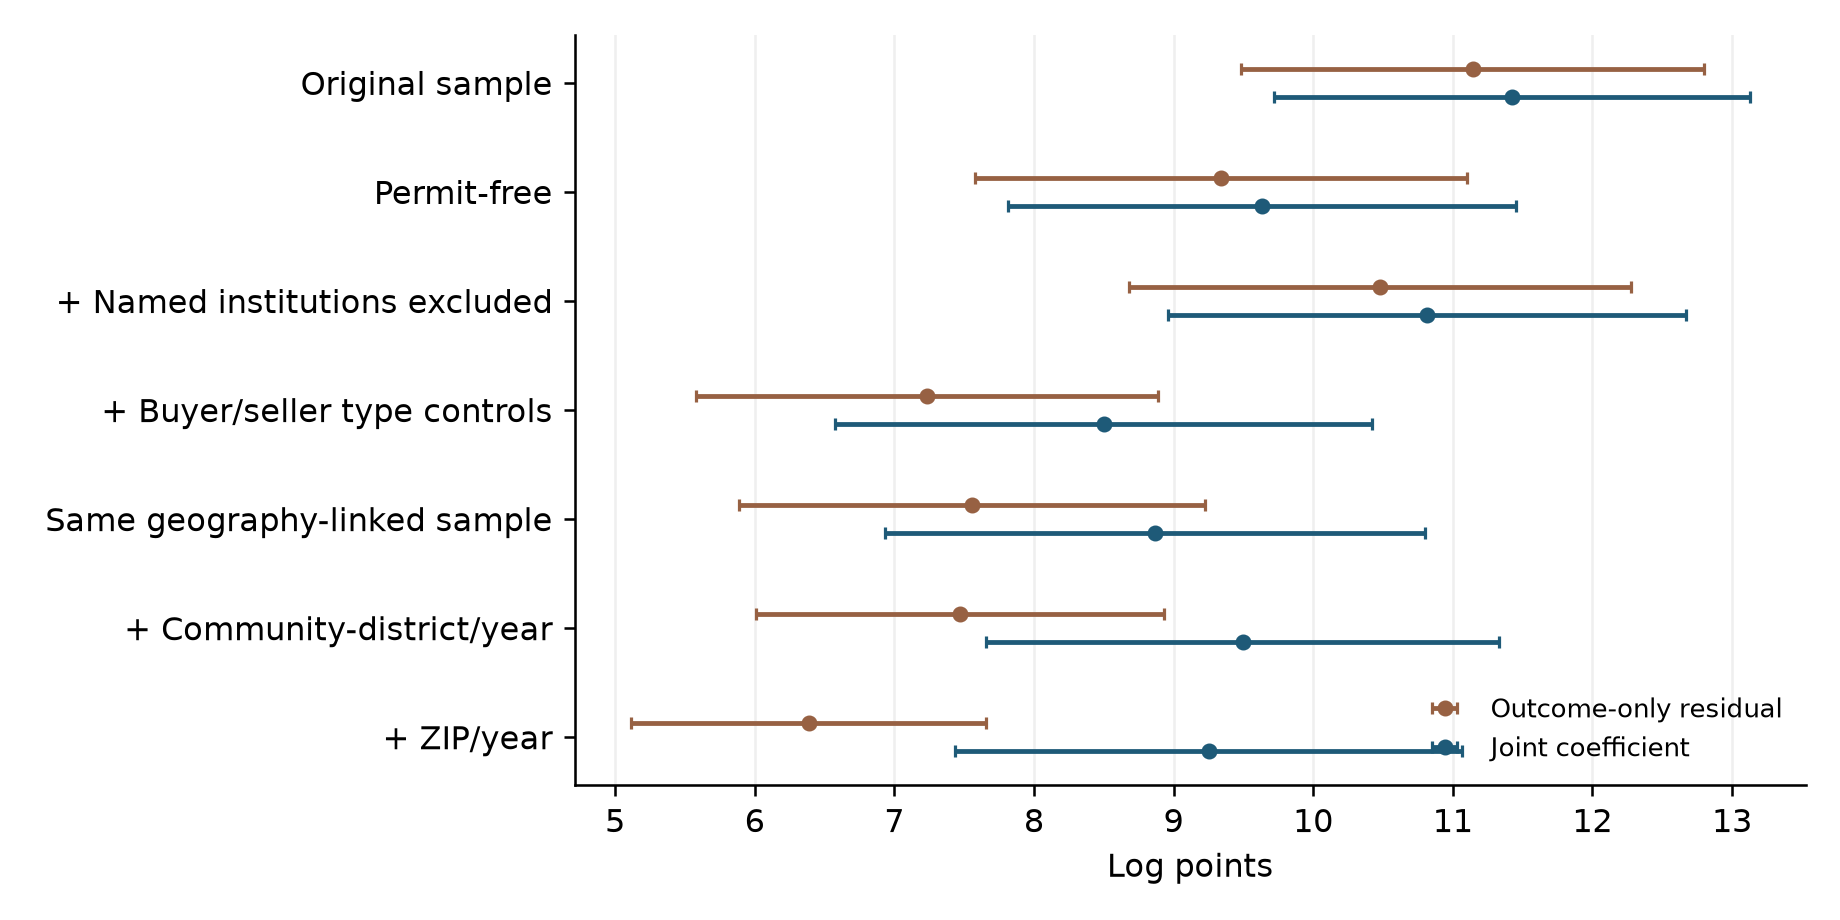
\includegraphics[width=\textwidth]{generated/robustness.png}
\caption{The residual-mean statistic and joint coefficient across controls}\label{fig:robustness}
\notes{Point estimates and pointwise parcel CR0 intervals. The figure uses one analytic interval method throughout; the principal table also reports common full-refit bootstrap intervals. Community-district/year and ZIP/year are alternative final controls.}
\end{figure}

All specifications' observation influences are summed within the original parcel and stacked before computing covariance. Excluded parcels receive zero influence in that specification. This preserves the covariance induced by overlapping samples. The 999-draw bootstrap resamples original parcel clusters and refits all nuisance controls in four principal specifications using the same draws. It confirms the main joint-coefficient comparison. The high-dimensional residual statistic has a shifted resampling distribution, another reason not to interpret its attenuation as an explained component. Intervals are pointwise and do not incorporate unobserved classification error.

\subsection{Outlier-robust estimates}\label{sec:robust}
The joint contrast is a mean, and repeat-sales growth has a long upper tail. In the headline sample, \TailCF{} percent of cash-to-financed pairs more than doubled in price, against \TailFF{} percent of pairs financed at both sales. Appendix Table~\ref{tab:focusedvalidation} shows the consequence: removing the 60 parcels with the largest positive influence, one percent of the sample, lowers the estimate to \FocusedPositive{} log points. Because that deletion selects on the fitted outcome, it has no valid sampling interpretation. Table~\ref{tab:robust} instead reports estimators fixed in advance that limit the weight of extreme growth without reference to the financing labels.
\begin{table}[htbp]\centering\footnotesize\setlength{\tabcolsep}{3pt}
\caption{Outlier-robust estimates of the financing contrast}\label{tab:robust}
\begin{tabular}{lrrrrr}\toprule
 & \multicolumn{3}{c}{Houses, full controls (6,006 pairs)} & \multicolumn{2}{c}{Borough-quarter only} \\
\cmidrule(lr){2-4}\cmidrule(lr){5-6}
Estimator & Contrast & 95\% CI & Change from LS & Houses & Condos \\
\midrule
Least squares (reference) & 9.25 & [7.17, 11.35] &  & 11.42 & 0.77 \\
Huber M-estimator & 6.73 & [5.32, 8.76] & -2.52 [-3.31, -1.14] & 8.83 & -0.49 \\
Trim growth at 1st/99th pct. & 7.66 & [5.77, 9.53] & -1.59 [-2.76, -0.45] & 9.23 & -0.45 \\
Trim growth at 2.5th/97.5th pct. & 5.15 & [3.55, 6.78] & -4.10 [-5.64, -2.53] & 6.91 & -0.58 \\
\bottomrule\end{tabular}
\notes{Log points. Columns 2--4 use the headline specification of Table~\ref{tab:cumulative} (ZIP-year and borough-quarter effects, buyer and seller type controls). Columns 5--6 use the common specification of Table~\ref{tab:property}. The Huber estimator ($k=1.345$; MAD scale from least-squares residuals, updated once) refits all nuisance controls by iteratively reweighted least squares. Trimming removes pairs whose annualized log growth lies outside the stated percentiles of the estimation sample; cutoffs ignore financing labels. Intervals are percentile intervals from the same 999 parcel-bootstrap draws as Table~\ref{tab:cumulative}, re-estimating the Huber scale and trimming cutoffs in every draw; the change column is the paired difference within draws. Tuning constants are conventional defaults and were not varied.}
\end{table}


The Huber estimator, which down-weights \RobustHuberDown{} percent of cash-to-financed pairs, gives \RobustHuber{} log points \RobustHuberCI{}. Trimming annualized growth at the 1st and 99th percentiles gives \RobustTrimOne{}, and at the 2.5th and 97.5th percentiles \RobustTrimTwo{}. For houses, every robust estimate is below least squares and every interval excludes zero. The house contrast remains positive under these alternative estimators, but its magnitude is sensitive to extreme appreciation. Under the common borough-quarter specification, the Huber estimate is \RobustHouseBQHuber{} \RobustHouseBQHuberCI{} for houses and \RobustCondoBQHuber{} \RobustCondoBQHuberCI{} for condominiums. The condominium contrast is much smaller and sensitive to the estimator, and the property-type divergence survives.

\subsection{Property types and classification sensitivity}
Table~\ref{tab:property} puts houses and condominiums under common borough-quarter controls. The condominium estimate is \CondoGap{} log points, with interval \CondoCI{}. Even with common controls, differences in ownership form, properties and matching coverage prevent attributing the contrast to standardisation or tax status alone.
\begin{table}[htbp]
\centering\small\singlespacing
\caption{House and condominium contrasts under common controls}\label{tab:property}
\begin{tabular}{lrrrrr}
\toprule
Type & Pairs & $N_{cf}$ & $N_{fc}$ & Joint & 95\% CI \\
\midrule
House & 8,208 & 1669 & 1035 & 11.42 & [9.72, 13.13] \\
Condo & 6,584 & 1228 & 1659 & 0.77 & [-0.01, 1.56] \\
\bottomrule
\end{tabular}
\notes{Both rows use borough-quarter effects and adjacent eligible sales at least 1,095 days apart. All available eligible pairs are used; the cumulative house restrictions are not imposed on the condominium sample. Parcel-clustered CR0 intervals, in log points. Differences in coverage, ownership and financing measurement prevent a causal property-type interpretation.}
\end{table}


The house findings survive narrower and wider financing windows, stable-label restrictions, broader institutional exclusions and consideration-consistent deed matching (Table~\ref{tab:sensitivity}). Window disagreement is an internal consistency measure. Among house sales, strict versus base labels differ for 1,020 observations and wide versus base for 2,193; neither is a known error count. Similarly, passing a consideration match does not establish distress status. A stratified instrument-review queue accompanies the code; no false-positive rate is inferred from these consistency checks.
\begin{table}[htbp]
\centering\small\singlespacing
\caption{Classification and linkage sensitivity}\label{tab:sensitivity}
\begin{tabular}{lrrr}
\toprule
Restriction & Pairs & Joint & 95\% CI \\
\midrule
Financing window: strict & 6,006 & 9.56 & [7.76, 11.36] \\
Financing window: base & 6,006 & 9.25 & [7.44, 11.07] \\
Financing window: wide & 6,006 & 8.60 & [6.77, 10.42] \\
Stable labels at both dates & 5,864 & 9.03 & [7.18, 10.88] \\
Broader institution exclusion & 5,918 & 9.31 & [7.48, 11.13] \\
Unique deed / amount match & 5,798 & 9.23 & [7.44, 11.02] \\
\bottomrule
\end{tabular}
\notes{All rows use the ZIP-year model, with borough-quarter and buyer/seller controls. Log points; parcel CR0 intervals. Stable labels agree between strict and wide windows at both dates. Amount consistency requires a unique nearest deed within 45 days and positive consideration within the larger of one dollar and one percent of the DOF price. These tests concern internal consistency, not classification accuracy.}
\end{table}


\section{Who pays cash?}\label{sec:who}
\subsection{Related-party transfers}
A sale between relatives can be recorded at any price and seldom needs a purchase mortgage. For a financing contrast such transfers are worse than noise. A below-market unfinanced sale at the first date raises measured appreciation in a cash-to-financed pair; one at the second date lowers it in a financed-to-cash pair. Both movements enlarge the half-difference, and they offset in the sum $A$ of equation~\eqref{eq:sym}, so the symmetry diagnostic cannot detect them.

The preserved ACRIS party extract names the grantors and grantees of the deed linked to each endpoint. Linked deeds with party records cover \PartyShareA{} percent of first-sale and \PartyShareZ{} percent of resale endpoints in the headline sample. A deed is flagged when a natural-person grantor and grantee share a surname, using names recorded in the `surname, given name' form; company, trust and estate names never match. The flag marks \RelPairs{} of the 6,006 pairs. Same-surname deeds are \RelRatio{} times as common at unfinanced endpoints (\RelShareCash{} percent) as at financed ones (\RelShareFin{} percent). Their prices are consistent with below-market transfers. Cash-to-financed pairs with a flagged deed have mean log appreciation of \RelGrowthCFRel{}, against \RelGrowthCFUnrel{} for other cash-to-financed pairs; flagged financed-to-cash pairs fall by \RelGrowthFCRel{} on average, while other financed-to-cash pairs rise by \RelGrowthFCUnrel{}.

Panel A of Table~\ref{tab:related} re-estimates the headline specification without flagged pairs. The house contrast falls to \NoRelOLS{} log points \NoRelOLSCI{}, a paired change of \NoRelChange{} \NoRelChangeCI{}. The Huber estimate falls to \NoRelHuber{} \NoRelHuberCI{}, and every estimator gives between \NoRelMin{} and \NoRelOLS{} log points. The flag makes two kinds of error. Unrelated parties can share a common surname: ignoring the 40 most frequent surnames in the extract removes most such coincidences and gives \NoRelStrictOLS{} \NoRelStrictOLSCI{}, although it also misses genuine relatives with common names. Relatives with different surnames, including many spouses and in-laws, are never flagged, and endpoints without party records cannot be flagged. The contrast that remains is therefore likely to contain some related-party transfers.

Every sampled deed carries a New York State real property transfer report (form RP-5217NYC), on which the parties declare the price and any condition of the transfer. A random sample of \DeedN{} flagged and \DeedUN{} unflagged cash-endpoint deeds (seed 20260924) was read from the ACRIS images with AI assistance, cross-checked against the transfer taxes paid, and confirmed by the author (Appendix~\ref{sec:deedreview}). \DeedYes{} of the \DeedN{} flagged deeds, \DeedShare{} percent \DeedCI{}, declare a sale between relatives or former relatives (\DeedBoxA{} deeds), a buyer who is also a seller, or a deed that is not a warranty or bargain-and-sale deed, or report a zero price with no transfer tax; \DeedPossible{} more combine a shared address or an owner on both sides with no declared condition. Among the unflagged cash deeds the share is \DeedUShare{} percent \DeedUCI{}. Declarations are self-reported and several flagged deeds between evident relatives declare no condition, so these shares are lower bounds on non-market transfers; the sample is too small to measure the flag's error rates precisely.
\begin{table}[htbp]\centering\footnotesize\setlength{\tabcolsep}{3pt}
\caption{Related-party transfers and the identity of the cash buyer}\label{tab:related}
\begin{tabular}{lrllrr}\toprule
\multicolumn{6}{l}{\textit{A. Financing contrast by estimator}}\\
Sample & Pairs & Least squares & Huber & Trim 1/99 & Trim 2.5/97.5 \\
\midrule
All pairs & 6,006 & 9.25 [7.17, 11.35] & 6.73 [5.32, 8.76] & 7.66 & 5.15 \\
No same-surname deeds & 5,648 & 4.87 [2.69, 6.76] & 4.02 [2.28, 5.73] & 4.03 & 2.83 \\
Same, strict flag & 5,768 & 6.71 [4.69, 8.72] & 4.94 [3.43, 6.79] & 5.13 & 3.06 \\
\midrule
\multicolumn{6}{l}{\textit{B. Least-squares contrast by the buyer at the cash sale}}\\
Sample & Pairs & Company buyer & Other buyer & \multicolumn{2}{r}{Other minus company} \\
\midrule
All pairs & 6,006 & 1.53 [-1.79, 5.44] & 13.77 [10.96, 15.98] & \multicolumn{2}{r}{12.24 [7.50, 16.06]} \\
No same-surname deeds & 5,648 & 1.55 [-1.75, 5.49] & 7.11 [4.48, 9.12] & \multicolumn{2}{r}{5.56 [0.97, 9.07]} \\
\bottomrule\end{tabular}
\notes{Log points; 95\% percentile intervals from the paper's 999 common parcel-bootstrap draws (seed 20260909), with every nuisance control, Huber scale and trimming cutoff re-estimated in each draw. Headline specification of Table~\ref{tab:cumulative}. A same-surname transfer is a deed at either endpoint on which a natural-person grantor and grantee share a surname; company, trust and estate names never match. The strict flag ignores the 40 most frequent surnames in the party extract. Panel B splits both switching arms by whether the grantee at the unfinanced sale has an explicit company form; always-financed and always-unfinanced pairs are pooled.}
\end{table}


\subsection{Company and individual cash buyers}
Panel B of Table~\ref{tab:related} splits both switching arms by the buyer at the unfinanced sale. Companies, identified by an explicit corporate form, are the cash buyer in \CashCompanyPairs{} of the \SwitchPairs{} switching pairs. When a company pays cash, the contrast is \CompanyCash{} log points \CompanyCashCI{}. When another party does, it is \OtherCash{} \OtherCashCI{}, and \OtherCashNoRel{} \OtherCashNoRelCI{} after excluding same-surname transfers. Even then the difference between the two groups is \OtherMinusCompanyNoRel{} log points \OtherMinusCompanyNoRelCI{}.

Companies that buy for cash are the investors most often described as outbidding financed households. In these data they pay close to what financed buyers pay for the same house. The price advantage is concentrated among individual cash buyers, and excluding pairs with same-surname deeds removes almost half of the headline contrast. The remaining gap among individuals is not thereby identified as a premium for certainty: individual cash purchases can also include estate sales, sales to tenants and other circumstances that names do not reveal. 
\subsection{Condominiums and a shared-address screen}
Deeds and parties were also retrieved for condominium endpoints, with every indexed request checked against the source's record count. A unique deed is linked for \CondoDeedEnds{} of \CondoEnds{} condominium endpoints; \CondoAmbiguous{} ambiguous matches are left unlinked. The same surname rule flags \CondoFlagged{} of 6,584 condominium pairs. Panel A of Table~\ref{tab:relatedext} applies the screen to both property types under the common borough-quarter design of Table~\ref{tab:property}. The house contrast falls from \InitialGap{} to \HouseBQNoRel{} log points \HouseBQNoRelCI{}; the condominium contrast moves from \CondoGap{} \CondoBootCI{} to \CondoNoRel{} \CondoNoRelCI{}, a paired change of \CondoRelChange{} \CondoRelChangeCI{}. Ignoring the 40 most common condominium surnames gives \CondoNoRelStrict{} \CondoNoRelStrictCI{}. Screening both property types therefore leaves the divergence between them intact.

A second proxy uses the mailing addresses recorded for each party. Panel B of Table~\ref{tab:relatedext} additionally excludes \AddrPairs{} house pairs with a deed on which the grantor and grantee share a normalized street address, city and ZIP code. The contrast falls to \AddrOLS{} log points \AddrOLSCI{}, but the additional change of \AddrChange{} \AddrChangeCI{} is not distinguishable from zero, and restricting the match to natural persons gives \AddrPersonOLS{} \AddrPersonOLSCI{}. Shared addresses are about as common at unfinanced endpoints (\AddrShareCash{} percent) as at financed ones (\AddrShareFin{} percent) and include common mailing agents and co-located parties, so this screen is a broad sensitivity rather than evidence of kinship.
\begin{table}[htbp]\centering\footnotesize\setlength{\tabcolsep}{2pt}
\caption{The same-surname screen across property types, and a shared-address sensitivity}\label{tab:relatedext}
\begin{tabular}{lrlrll}\toprule
\multicolumn{6}{l}{\textit{A. Common borough-quarter design (Table~\ref{tab:property})}}\\
 & Pairs & All pairs & Flagged & Unflagged pairs & Change \\
\midrule
Houses & 8,208 & 11.42 [9.60, 13.19] & 449 & 7.50 [6.00, 9.19] & -3.93 [-4.81, -2.94] \\
Condominiums & 6,584 & 0.77 [-0.02, 1.55] & 189 & -0.46 [-1.16, 0.14] & -1.23 [-1.71, -0.82] \\
\midrule
\multicolumn{6}{l}{\textit{B. Headline house specification: excluding pairs with}}\\
 & Pairs & Contrast & \multicolumn{2}{l}{Change vs.\ surname screen} & \\
\midrule
Same-surname deeds & 5,648 & 4.87 [2.69, 6.76] & \multicolumn{2}{l}{} \\
\quad or shared address & 4,053 & 3.76 [1.16, 6.05] & \multicolumn{2}{l}{-1.11 [-2.76, 0.29]} \\
\quad or shared address, persons & 4,458 & 4.41 [2.14, 6.75] & \multicolumn{2}{l}{-0.46 [-1.43, 0.71]} \\
\bottomrule\end{tabular}
\notes{Log points; 95\% percentile intervals from the paper's 999 common parcel-bootstrap draws (seed 20260909), refitting all controls in each draw. Panel A: least squares under borough-quarter effects only, as in Table~\ref{tab:property}; the same-surname flag of Table~\ref{tab:related} is applied to deeds linked to each endpoint. Condominium deeds are linked for 13,092 of 13,168 endpoints (31 ambiguous matches left unlinked). Panel B: headline specification of Table~\ref{tab:cumulative}. A shared address is a grantor and grantee on the same deed with the same normalized mailing street, city and ZIP code; it can reflect a common mailing agent or co-location and is not evidence of kinship. The natural-person variant counts only addresses of parties with personal names.}
\end{table}


\section{Interpreting the financing gap}
\subsection{What the magnitudes imply}
Consider a stylised seller comparing a certain cash price $P_c$ with a financed offer $P_f$. Let $q$ be the probability that the financed transaction fails and let $dP_c$ be the loss, relative to the cash alternative, conditional on failure. If continuation following failure is worth $(1-d)P_c$, indifference implies
\begin{equation}
P_c=(1-q)P_f+q(1-d)P_c,
\qquad \frac{P_f-P_c}{P_c}=\frac{qd}{1-q}.
\end{equation}
For an observed log contrast $\pi$, treating that entire contrast as the model premium requires
\begin{equation}\label{eq:inverse}
d^*(q;\pi)=(e^\pi-1)\frac{1-q}{q}.
\end{equation}
This inversion makes the required loss explicit while leaving $q$ as an assumption. Mortgage application denial is not the failure probability of an accepted purchase contract, so national denial rates are not substituted for $q$ here.
\begin{table}[htbp]
\centering\small\singlespacing
\caption{Relisting-loss scenarios implied by the observed contrasts}\label{tab:inversion}
\begin{tabular}{lrr}
\toprule
Failure probability $q$ & Houses: $100d^*$ & Condos: $100d^*$ \\
\midrule
0.1 & 87.2 & 7.0 \\
0.2 & 38.8 & 3.1 \\
0.3 & 22.6 & 1.8 \\
\bottomrule
\end{tabular}
\notes{Scenario calculations from $d^*=(\exp(\pi)-1)(1-q)/q$. Houses use the full geographic joint estimate; condos use the borough-quarter joint estimate. They have different covariate sets and populations. Values of $q$ are illustrative assumptions, not estimated contract-failure probabilities. No common relisting technology is imposed as an empirical fact.}
\end{table}


At any common failure probability, the house contrast implies a loss on failure more than ten times as large as the condominium contrast if the entire gap is attributed to execution risk. At an assumed $q=0.1$, it would require a continuation loss of 87 percent of the price, or \RobustHouseInvQTen{} percent at the Huber estimate, compared with about 7 percent for condominiums (and zero or negative under robust condominium estimates). Without same-surname pairs the house requirement falls to \NoRelInvQTen{} percent, or \NoRelHuberInvQTen{} percent at the Huber estimate, which is still several times the condominium figure; the screened condominium contrast requires no loss at all. A seller whose financed buyer fails still owns the house and can relist it. While a loss of a few percent aligns with ordinary carrying and relisting costs, a loss exceeding half the property's value illustrates the extreme demands that an execution-risk explanation places on the house contrast. These calculations illustrate model requirements under stated assumptions rather than estimating the actual mechanism share, because contract failure rates and continuation values are unobserved.

Two qualifications apply. First, equation~\eqref{eq:inverse} evaluates the counterfactual in which the entire observed contrast represents a causal financing premium, which the design does not establish. The calculation evaluates what execution risk would have to explain under that assumption, rather than bounding or estimating the true closing-risk contribution. Second, failure probabilities could differ between the two property types. To reconcile the least-squares contrasts with a common loss, the failure odds would have to be about twelve times higher for houses than for condominiums. The mechanism in \citet{hanhong2024}, where market-specific relisting prospects interact with closing risk, is the natural candidate for such a difference and would require contract-level data to test.

\subsection{What the co-operative comparison can establish}
Co-operative share financing is a possible institutional comparison, but the recorded loan measure differs from the house and condominium measure. Timing-unique filing assignments leave 1,765 repeat pairs with an interval including zero; an instrument pilot nevertheless finds a filing that pledges a different unit from its assigned sale. That sale contributes no repeat pair, so rejecting its link leaves the estimate unchanged. A second filing matches the sale unit but lacks independent confirmation of purchase-loan purpose. Appendix~\ref{sec:coopaudit} reports the full assignment and adjacency audit. The co-operative comparison is therefore a measurement sensitivity, not a control group that identifies a mortgage-tax effect.

\subsection{Credit conditions at both sale dates}
If credit conditions shape financing risk, attaching a rate only to the resale misses conditions at the initial transaction. The full house design therefore adds separate terms $F_a(r_a-4)$ and $F_z(r_z-4)$, where $r$ is the latest available weekly Freddie Mac 30-year PMMS rate, in percent, on or before each sale. Quarterly effects do not absorb all within-quarter weekly-rate variation. Separate uninteracted rates at both endpoints are therefore included explicitly. The exercise studies financing-specific rate associations.

The slopes are small and negative at the first date and positive at the second date (Table~\ref{tab:credit}). Adding separate financing-specific linear calendar trends reverses both signs; the two rate interactions are not jointly distinguishable from zero in the calendar-dependence sensitivity (Appendix Table~\ref{tab:marketconditions}). Rate movements, time trends and financing composition are difficult to disentangle in these data. The rate evidence consequently does not identify the execution-risk mechanism. The PMMS methodology change on 17 November 2022 is an additional measurement qualification. The augmented model's reference contrasts at 4 percent and the trend origin must not be reported as an unconditional average financing gap.
\begin{table}[htbp]\centering\small
\caption{Credit conditions at both sale dates}\label{tab:credit}
\begin{tabular}{lrrrr}\toprule
Financing $\times$ rate & Without trends & SE & With trends & SE \\
\midrule
First sale & -0.43 & 1.95 & 0.46 & 1.93 \\
Second sale & 2.98 & 0.62 & -1.24 & 1.03 \\
\bottomrule\end{tabular}
\notes{Log points per one percentage point of PMMS rates, centered on 4 percent; 6,006 pairs. Both models include separate uninteracted weekly rates at both endpoints, the full geographic controls and both financing-switch indicators. The second adds separate endpoint financing-specific linear calendar trends. Standard errors cluster by parcel (CR0). Appendix Table~\ref{tab:marketconditions} reports calendar-dependence sensitivity. The headline contrast is estimated in the model without rate interactions.}
\end{table}


A bounded extension attaches prior-month borough inventory to both sale dates using StreetEasy's Single Family series \citep{streeteasy2026}. All 6,006 house pairs are covered. The resale-date financing interaction reverses sign when financing-specific trends are added, and the joint calendar-quarter test then does not reject zero endpoint interactions. Appendix~\ref{sec:marketconditions} reports both specifications. This sensitivity does not isolate a liquidity or execution-risk mechanism.

\section{Conclusion}\label{sec:conclusion}
In New York City, financed purchases of houses are associated with prices \HouseGap{} log points above cash purchases of the same house, and between \RobustMin{} and \RobustMax{} log points under estimators that limit the weight of extreme appreciation. That average conceals who pays cash. Company cash buyers pay about what financed buyers pay. The discount sits with individual cash buyers, and excluding pairs with a deed on which the seller and buyer share a surname reduces the house contrast by almost half, to \NoRelOLS{} log points \NoRelOLSCI{}. Screened the same way, condominium contrasts are close to zero, while houses retain a clear positive contrast. Under a simple seller indifference model with an assumed 10 percent failure probability, even the reduced house contrast would require a loss of \NoRelInvQTen{} percent of the price on a failed sale to be a pure premium for execution certainty, against about 7 percent for condominiums.

These conclusions rest on measured, not verified, transaction attributes. Financing labels come from matching purchase-window mortgages and are not confirmed loan purposes; the absence of a match is not proof of a cash purchase. A shared surname or mailing address is a proxy for a relationship, not proof of one: it misses relatives with different names and can match unrelated people. Transfer reports in a small random sample of deed images, read with AI assistance and confirmed by the author, show non-market signs in \DeedShare{} percent of flagged deeds and \DeedUShare{} percent of other cash deeds; these declarations are self-reported and the sample is small. Permits capture recorded renovation, not all changes in condition. Institutional-name rules mix foreclosure transfers with lender resales and cannot establish distress. Co-operative financing assignments rely on timing and can attach a filing to the wrong unit. The panel's record linkage is archived and documented but was not rebuilt from raw records for this version. A blinded, probability-sampled review of the underlying instruments has been prepared but not yet completed (Appendix~\ref{sec:focusedvalidation}). All reported intervals condition on these measurements.

For policy, the results caution against reading an observed cash--mortgage price difference as the value of closing certainty or as the advantage of investors who pay cash. In these data, little of the gap belongs to company buyers, and a measure that includes family transfers is a poor basis for any tax or subsidy rate on the payment method. In May 2026, New York legislators considered, and then dropped from the state budget, a buyer-paid tax of 1 percent on New York City home purchases of \$1 million or more made without a mortgage, presented as parity with the mortgage recording tax \citep{bloomberg2026cashtax,bloomberg2026cashtaxdropped}. The results here do not evaluate that proposal, which would apply only above \$1 million, but they caution against justifying such a tax by an observed cash discount. Research that uses administrative financing labels should screen related-party transfers before interpreting a cash discount. Separating execution risk from selection requires data on accepted offers, contingencies, failed closings and relisting, or an exogenous source of financing variation. The statutory mortgage recording tax is a distinct and directly measurable cost to financed buyers; its size and the design of New York's transfer-tax thresholds are examined in \citet{loschi2026shape}.

\section*{Declarations}\begingroup\small\singlespacing
\noindent\textbf{Data availability.} All inputs are public records of New York City agencies and Freddie Mac. Code, archived inputs, preserved public extracts and complete outputs are deposited at \href{https://doi.org/10.5281/zenodo.22421850}{doi:10.5281/zenodo.22421850} (concept DOI, resolving to the current version). A master script regenerates every table and figure from those files; the replication README documents the one stage not re-executed, the original raw-to-panel linkage.

\noindent\textbf{Funding and interests.} Sole author; independent researcher. There was no external funding. The author reports no relevant financial interests or positions and no outside rights to review the research before dissemination.

\noindent\textbf{Prior dissemination.} Earlier versions circulated as a working paper (SSRN 7421138) and with the replication deposit. The paper is not under review elsewhere.

\noindent\textbf{Generative AI.} AI tools assisted with drafting, literature checking, code development and replication review. The author is responsible for the manuscript, interpretations and citations. This statement does not certify independent human verification of unresolved instrument classifications. The research uses administrative public records; no human subjects were involved.

\par\endgroup\clearpage\appendix
\section{Joint uncertainty and numerical implementation}
Write $r=M_Xy$ and $m=M_Xc$. The derivative of the residual contrast with respect to an observation weight, evaluated at unit weights, is
\begin{equation}
\operatorname{IF}_{R,i}=m_i r_i-\frac{1\{cf\}_i\bar r_{cf}}{2N_{cf}}+\frac{1\{fc\}_i\bar r_{fc}}{2N_{fc}}.
\end{equation}
The first term accounts for refitting the nuisance projection; the remaining terms account for changes in group denominators. For the joint estimator, let $R=M_XQ$ and $e=M_Xy-R\widehat\beta$. Its coefficient derivative is
\begin{equation}
\operatorname{IF}_{\beta,i}=(R'R)^{-1}R_i'e_i.
\end{equation}
Apply the half-difference contrast, sum within parcel and stack across specifications. The covariance is the cross-product of these stacked cluster influences (CR0). Paired-difference variances use the corresponding covariance terms, rather than treating the two estimates as independent.

A numerical check perturbs five actual parcel weights in the full ZIP-year model, refits the nuisance parameters and verifies both analytic derivatives against finite differences with absolute error below $10^{-7}$. The common bootstrap draws multinomial weights over the 8,127 original house parcels, using seed 20260909, and refits the original, permit-free, linked-party-control and ZIP-year specifications. All 999 draws are retained. Redundant nuisance columns are projected out without interpreting an arbitrary individual fixed-effect solution.

No multiple-testing correction is applied; all intervals are pointwise. These covariance calculations condition on the observed linkage and classifications.

\section{Replication map and classification definitions}
The master script \texttt{code/reproduce.py} parses the preserved rate extracts, rebuilds enriched pairs, estimates the house models and bootstrap, audits co-operative assignments, estimates the outlier-robust models, performs numerical checks and regenerates manuscript exhibits. The replication README contains exact setup instructions, package versions and a file-level exhibit map. Archived original inputs remain distinguishable from newly retrieved extracts and derived outputs.

Table~\ref{tab:cumulative}, Table~\ref{tab:paired} and Figure~\ref{fig:robustness} derive from the repeat-sale results and joint bootstrap outputs. Table~\ref{tab:property} recomputes both property types from the archived panel. Table~\ref{tab:robust} is produced by \texttt{code/robust\_estimators.py} from the same parcel-bootstrap draws. The co-operative, credit and classification tables map to their named analysis scripts. Table~\ref{tab:inversion} is computed directly from the displayed formula and identified point estimates.

The loan windows in the house/condominium input are document-based purchase-window proxies; the co-operative windows concern personal-property recording dates. These do not have identical coverage or timing interpretation. The party classifications are reproducible regular-expression categories, not verified persons, beneficial owners or distressed sales. Unknown party records remain explicit rather than being silently classified as individuals. The release retains audit fields and review queues so subsequent adjudication can be versioned without overwriting the underlying rules.


\section{Co-operative assignment and adjacency audit}\label{sec:coopaudit}
\subsection{Why the co-operative comparison requires an audit}
A building-level UCC filing is not inherently a particular unit buyer's purchase loan. Multiple sales and filings can occur near each other, some sales lack recovered unit identifiers, and filings can concern other credit events. The co-operative extract therefore includes all observed prices and incomplete-unit records when counting possible competitors for a filing, rather than using only the estimation sample.

The broadest rule, the expanded count rule, works as follows: for a sale at date $d$, count eligible sales within $d\pm45$ days and filings within $[d-60,d+135]$. A zero filing count is coded cash; a filing count at least as large as the sale count is coded financed; the remainder is ambiguous. The expansion is consequential. Of 60,496 purchases labelled financed, 4,385 have no filing in the base $[-15,+90]$-day window. Counting all observed competing sales also changes assignments.

The alternative rules require exactly one candidate filing and exactly one observed sale eligible to claim that filing. The narrow, base and wide windows are $[-15,+30]$, $[-15,+90]$ and $[-15,+180]$ days. Documents linked to multiple parcels are excluded. These conditions prevent reuse of a supposedly unique filing, but cannot identify its debtor, collateral unit or purchase purpose. Zero candidates still means no matched record, not proven cash.

Adjacency is determined using all observed known-unit sales before dropping endpoints with ambiguous financing or out-of-band prices. Forming pairs within the estimation sample alone would bridge an intervening observed unit sale in 271 cases, so Table~\ref{tab:coop} forms adjacency on all known-unit sales in every row. Base timing uniqueness leaves 1,765 pairs in 1,082 buildings. Its interval includes zero, as do the narrow and wide alternatives. This is compatible with a small co-operative contrast within selected, differently measured samples; it is not evidence that the mortgage recording tax causes the house gap.
An instrument pilot makes the remaining linkage problem concrete. Among two timing-unique candidates inspected, one filing names the recorded sale unit; the other pledges a different unit in the same building. The latter sale contributes no repeat pair, so rejecting its filing link does not change Table~\ref{tab:coop}. The matching case still lacks independent confirmation of purchase-loan purpose. These observations demonstrate a failure mode, not a population error rate, and preclude treating timing uniqueness as validated financing.
\begin{table}[htbp]
\centering\small\singlespacing
\caption{Co-operative assignment sensitivity}\label{tab:coop}
\begin{tabular}{lrrrrr}
\toprule
Assignment rule & Pairs & $N_{cf}$ & $N_{fc}$ & Joint & 95\% CI \\
\midrule
Expanded count rule & 5,839 & 247 & 602 & -1.18 & [-3.11, 0.75] \\
All competing sales & 5,261 & 229 & 576 & -0.89 & [-2.77, 1.00] \\
Unique timing: narrow & 2,840 & 441 & 537 & -0.41 & [-2.00, 1.18] \\
Unique timing: base & 1,765 & 219 & 252 & -1.42 & [-3.70, 0.86] \\
Unique timing: wide & 1,265 & 108 & 143 & 0.09 & [-2.99, 3.17] \\
\bottomrule
\end{tabular}
\notes{Log points and building-clustered CR0 intervals. Every row forms adjacency using all observed known-unit sales before dropping ineligible endpoints and ambiguous financing. Timing uniqueness does not establish debtor identity or purchase purpose. No matched filing is a cash proxy, not proof of an unlevered purchase. Estimates use the September 2026 co-operative extract.}
\end{table}



\section{Targeted instrument pilot}\label{sec:pilot}
Four queued cases were inspected through the public ACRIS image viewer on 10 September 2026: one broad-only house flag, one specific-institution house flag, and two timing-unique co-operative assignments. Saved page images, document identifiers, review notes and source hashes accompany the replication package. These are AI-assisted document readings awaiting independent review. The 90-house and 90-co-operative queues remain incomplete; their sampling weights must not be applied to this selectively continued four-case pilot to estimate error rates.

House deed 2023051600851001 recites the lender's acquisition under referee deed 2019020500740001. The earlier operative instrument describes a mortgage foreclosure and conveyance to the lender; the later transaction is consistent with a lender resale. The broader name rule flags the sale whereas the narrower rule does not. House deed 2019093000695001 is explicitly a referee's deed in foreclosure and is already caught by the narrower institutional-buyer rule. Both source cover records use DEED metadata. These findings distinguish mechanisms within institutional flags without measuring property condition or the effect of distress on prices.

For co-operative filing 2025020500312001, the sale unit and collateral designation both identify 7AB, but purchase-loan purpose remains unverified. Filing 2020020400882001 pledges unit 4E, whereas its timing-assigned sale identifies 1CD. The preserved sale extract contains only one observation for that latter unit; the false link therefore affects no repeat pair. It is rejected as evidence for that sale's financing, without relabelling the sale as cash. A timing-only rule cannot resolve this unit mismatch even when it has no observed competing sale.

\section{Historical market conditions and shared calendar shocks}\label{sec:marketconditions}
The inventory extension uses one selected indicator: the log base two of StreetEasy's prior-month borough sales inventory in its Single Family category. It is centered on each borough's unweighted mean log inventory over December 2015--November 2025, so a unit represents a doubling relative to that reference. The downloaded September 2026 vintage covers both endpoints of all 6,006 pairs. Its listing coverage need not represent the administrative one-to-three-family house sample. Inventory reflects both supply and demand, including platform participation; it is not a direct measure of closing risk. Historical revisions and unknown publication dates mean that a prior-month observation is not necessarily information publicly available on the sale date.

Both endpoint inventory levels enter uninteracted, alongside separate financing-inventory interactions, the full house controls, and endpoint financing-by-borough controls with Brooklyn omitted. The latter prevent fixed geographic differences in financing associations from being attributed to inventory movements. Separate financing-specific linear calendar trends are then added as a sensitivity. This plan was recorded after checking source coverage and before fitting these associations; it was not externally preregistered. Both fitted specifications are reported, without choosing a preferred indicator or trend specification from significance.

\begin{table}[htbp]\centering\small
\caption{Historical market conditions: endpoint and trend sensitivity}\label{tab:marketconditions}
\begin{tabular}{lrrrrrr}\toprule
Model & First & 95\% CI & Second & 95\% CI & $p_Q$ & $p_Y$ \\
\midrule
Credit & -0.43 & [-5.91, 5.05] & 2.98 & [2.02, 3.94] & $<0.001$ & $<0.001$ \\
Credit + trends & 0.46 & [-4.63, 5.54] & -1.24 & [-3.18, 0.70] & 0.418 & 0.330 \\
Inventory & -3.13 & [-7.17, 0.91] & -13.38 & [-22.54, -4.21] & 0.005 & 0.003 \\
Inventory + trends & -4.51 & [-9.79, 0.77] & 3.21 & [-6.65, 13.08] & 0.195 & 0.244 \\
\bottomrule\end{tabular}
\notes{All 6,006 pairs; slopes in log points. Credit unit: one percentage point of the weekly rate. Inventory unit: a doubling of prior-month borough Single Family inventory relative to its borough reference. Inventory models also include separate endpoint financing-by-borough controls (Brooklyn reference). Both indicators enter uninteracted at both dates. Intervals use the union of parcel and either-endpoint calendar-quarter score dependence and a $t_{39}$ reference. Columns $p_Q$ and $p_Y$ test both interaction slopes jointly, using calendar-quarter and calendar-year dependence respectively, with approximate $F_{2,39}$ and $F_{2,9}$ references. Negative covariance eigenvalues are set to zero: one is corrected in each quarter model with trends and in each year model. The unadjusted eigenvalues are recorded in the replication output. These are exploratory, pointwise diagnostics, not exact small-cluster inference.}
\end{table}


Parcel-only uncertainty is supplied in the replication output. The table additionally allows score dependence whenever two repeat pairs share a parcel or either endpoint calendar period, regardless of whether the shared period belongs to their first or second sales. Inclusion--exclusion counts overlapping memberships once. The calendar-quarter calculation uses 40 nodes; the calendar-year sensitivity uses only ten. Negative eigenvalues in the estimated covariance are replaced by zero, with their magnitudes retained in the output. The resulting $t$ and $F$ references are approximate diagnostics, not exact small-cluster tests. These calculations do not cover arbitrary dependence across non-overlapping periods, and intervals are pointwise without multiplicity adjustment.

With trends, the inventory interactions are not jointly distinguishable from zero under either calendar aggregation. The analogous credit exercise reaches the same qualitative conclusion after common weekly rates are included. This does not demonstrate that market conditions are irrelevant; it shows that these associations are sensitive to their time specification. The headline conditional house contrast is estimated in the unchanged main model and is not replaced by the reference contrast from either interaction model.


\section{Deed-image review of the same-surname flag}\label{sec:deedreview}
The review sample was drawn by an independent audit before any deed was read: \DeedN{} endpoint deeds at random among flagged pairs and \DeedUN{} among unflagged cash endpoints of the headline house sample (seed 20260924). All 684 pages of the 60 recorded documents were retrieved from the public ACRIS image service. Each contains a cover page, the deed, and a New York State real property transfer report (RP-5217NYC). Item 12 of that report gives the full sale price and item 14 lists conditions of the transfer, including (A) a sale between relatives or former relatives, (C) a buyer who is also a seller and (E) a deed type other than warranty or bargain and sale. Prices and conditions were read from the report images; cover pages supplied the parties' addresses and the city and state transfer taxes, whose rates imply the taxed consideration. Where the report price and the taxed consideration disagree, both are recorded and the case is classed as unclear rather than resolved. Readings were made with AI assistance, documented deed by deed, and confirmed by the author; the readings, image crops and scripts are in \texttt{audit/deed\_image\_review}.

A deed is classed as showing a non-market sign when it declares condition A, C or E, or reports a zero price with no transfer tax. The classification is conservative. Conditions are self-declared: a transfer from a father to a son of the same name, for instance, declares none. Among flagged deeds, \DeedPossible{} further cases list a buyer among the sellers or give the same address for both parties without declaring a condition. One flagged deed shares only a common surname among seven parties and is dropped by the strict flag, and one unflagged deed declares a sale between relatives with different surnames. The review therefore supports the flag as a marker of non-market transfers without measuring its sensitivity or specificity.

\section{Focused validation of the house contrast}\label{sec:focusedvalidation}
A bounded validation pass checks the exact archived rows generating the 6,006 analysis pairs. There are 5,957 parcels and 11,963 distinct sale endpoints. All pair price changes and financing flags reconstruct from those rows, and the three financing windows are nested. The linear coefficient weights reproduce the joint house contrast to numerical precision. These checks establish computational consistency, not the correctness of the archived source linkage.

Ten pairs involve an endpoint with more than one house record on the same parcel and date. Three financed sale endpoints have no positive recorded mortgage amount. Neither finding proves a false sale or financing classification, but both warrant explicit scrutiny. Omitting these cases and applying the existing safeguards jointly leaves 5,579 pairs and a contrast of \FocusedJoint{} log points. The archived house panel does not retain the mortgage instrument identifiers needed for independent purchase-loan verification.

Table~\ref{tab:focusedvalidation} reports the complete refitted sequence.
\begin{table}[htbp]\centering\small
\caption{Focused house validation: influence, geography and source consistency}\label{tab:focusedvalidation}
\begin{tabular}{lrrr}\toprule
Restriction & Pairs & Contrast & Change \\
\midrule
Main reference & 6,006 & 9.25 & +0.00 \\
Omit top 1 absolute influences & 6,005 & 9.07 & -0.18 \\
Omit top 5 absolute influences & 6,001 & 9.68 & +0.42 \\
Omit top 10 absolute influences & 5,996 & 9.79 & +0.54 \\
Omit top 30 absolute influences & 5,976 & 9.41 & +0.16 \\
Omit top 60 absolute influences & 5,946 & 8.51 & -0.74 \\
Omit 60 largest positive influences & 5,946 & 4.68 & -4.57 \\
Omit Manhattan & 5,962 & 9.26 & +0.01 \\
Omit Bronx & 4,962 & 9.42 & +0.17 \\
Omit Brooklyn & 4,052 & 10.39 & +1.14 \\
Omit Queens & 3,042 & 7.91 & -1.34 \\
Omit ZIP 11234 & 5,801 & 9.11 & -0.14 \\
Omit ZIP 10465 & 5,844 & 9.01 & -0.25 \\
Omit ZIP 11357 & 5,875 & 9.25 & -0.00 \\
Joint record-consistency safeguards & 5,585 & 8.98 & -0.27 \\
Omit ambiguous source dates & 5,996 & 9.29 & +0.04 \\
Omit missing positive loan amounts & 6,003 & 9.25 & -0.00 \\
Joint safeguards and source checks & 5,579 & 9.02 & -0.23 \\
\bottomrule\end{tabular}
\notes{Log points. Every row refits the joint switch model and all nuisance controls on its retained sample. Parcels, not single observations, are removed in the influence exercises. Absolute- and positive-influence exclusions are selected using the fitted outcome; they are diagnostics, not alternative preferred samples, and ordinary confidence intervals would not account for that selection. Geographic and source restrictions also change the estimation population. The three ZIPs are selected by pair count. Combined safeguards require stable financing windows, unique amount-consistent deeds at both endpoints and no broad institutional-name flag. Source checks additionally remove ambiguous parcel/date records and financed endpoints without positive recorded loan amounts. These are internal consistency restrictions, not validated classifications. The complete model outputs and nominal parcel intervals are retained in the replication files.}
\end{table}


Influence is calculated from the fitted joint model and aggregated by parcel. Every deletion refits all nuisance controls. Removing the single largest absolute-influence parcel leaves 9.07 log points; the 60-parcel absolute-influence deletion leaves \FocusedTopSixty{}. This argues against a single-record explanation. It does not establish insensitivity to adversarial sample selection: removing the 60 largest positive influences lowers the estimate to \FocusedPositive{}. Section~\ref{sec:robust} addresses the same concern with robust estimators using conventional tuning constants that have valid intervals. Omission of each borough and each of the three largest ZIP groups is reported, without selecting the most favorable comparison.

The replication output also reports adversarial perturbations to pair log-price growth, holding the labels and design fixed. It selects parcels with the largest absolute coefficient-weight sums and moves their outcomes against the weight signs. These exact linear calculations quantify sensitivity to outcome contamination under stated assumptions. They are not financing-misclassification bounds or estimates of unobserved renovation effects.

A price-blinded review queue samples 20 pairs at random from each financing-switch arm, separately from targeted influential and missing-amount cases. The analyst key preserves strata and inclusion probabilities; the reviewer file omits price changes, financing predictions and influence ranks. No independent human instrument reviews have been completed in this new queue, and no population error rate is estimated. Review of the operative deed and mortgage instruments remains necessary to determine borrower, collateral and purchase-financing consistency. Absence of a matched loan cannot certify cash financing.

\clearpage
\begingroup\small\singlespacing\raggedright\bibliography{references}\endgroup
\end{document}
